% Selection flow (counts as stated in Sec. I, "Paper selection" paragraph). Plain TikZ.
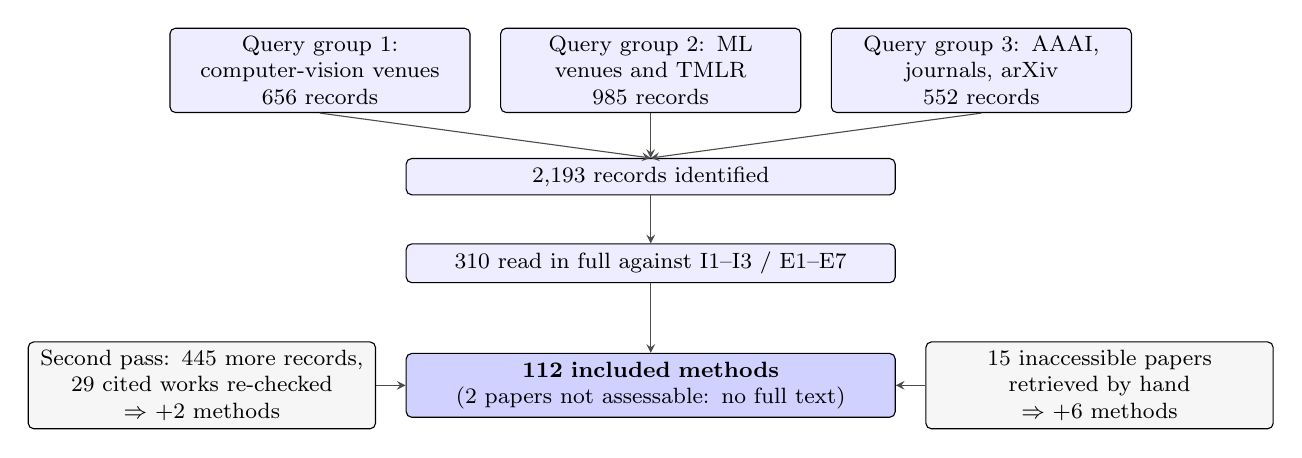
\begin{tikzpicture}[x=1cm, y=-1cm, font=\footnotesize,
  box/.style={draw, rounded corners=2pt, fill=blue!7, align=center, inner sep=3pt, text width=#1},
  box/.default=3.6cm, side/.style={draw, rounded corners=2pt, fill=gray!7, align=center, inner sep=3pt, text width=4.2cm},
  ar/.style={->, >=stealth, black!70, thin}]
  \node[box=3.6cm] (s1) at (0,0)   {Query group 1: computer-vision venues\\656 records};
  \node[box=3.6cm] (s2) at (4.2,0) {Query group 2: ML venues and TMLR\\985 records};
  \node[box=3.6cm] (s3) at (8.4,0) {Query group 3: AAAI, journals, arXiv\\552 records};
  \node[box=6cm]   (id) at (4.2,1.35) {2,193 records identified};
  \node[box=6cm]   (ft) at (4.2,2.45) {310 read in full against I1--I3 / E1--E7};
  \node[box=6cm, fill=blue!18] (in) at (4.2,4.0) {\textbf{112 included methods}\\(2 papers not assessable: no full text)};
  \node[side] (p2) at (-1.5,4.0) {Second pass: 445 more records,\\29 cited works re-checked\\$\Rightarrow$ +2 methods};
  \node[side] (hand) at (9.9,4.0) {15 inaccessible papers\\retrieved by hand\\$\Rightarrow$ +6 methods};
  \foreach \s in {s1,s2,s3} \draw[ar] (\s.south) -- (id.north);
  \draw[ar] (id) -- (ft); \draw[ar] (ft) -- (in);
  \draw[ar] (p2) -- (in); \draw[ar] (hand) -- (in);
\end{tikzpicture}
